\documentclass[11pt,letterpaper, oneside, headings=normal,final]{article}


\usepackage[paper=a4paper,left=2cm,right=2cm,top=2.5cm,bottom=2cm]{geometry}
\usepackage[english,ngerman]{babel}
\usepackage[T1]{fontenc}
\usepackage[latin1]{inputenc}
\usepackage{verbatim}

\usepackage{ifthen}
\usepackage{fancyhdr}
\usepackage{color}

\usepackage{placeins}
\usepackage{amssymb}
\usepackage{amsmath} 
\usepackage{graphicx}

\usepackage[colorlinks=true, allcolors=blue]{hyperref}
\usepackage[figure,table]{hypcap}

\usepackage{pgf,tikz}
\usepackage{mathrsfs}
\usepackage{setspace}
\usetikzlibrary[patterns]
\usepackage{pdfpages}

\usepackage{multirow}
%%%%%%%%%%%%%%%%%%%%%%%%%%%%%%%%%%%%%%%%%%%%%%%%%%%%%
% Farben f�r Hyperlinks z.B.
\definecolor{lt_gray}{rgb}{.8,.8,.8}
\definecolor{red}{rgb}{.90196,.0,.2}
%\definecolor{green2}{rgb}{0,.5,.0}
%\definecolor{myblue}{rgb}{.27,.51,.71} % 69 130 181
\definecolor{myblue}{rgb}{0,.5,.0}
\definecolor{green2}{rgb}{.27,.51,.71}
%
\newcommand{\Th}{\mathcal{T}_h}
\newcommand{\OmegaBg}{\widehat{\Omega}}
\newcommand{\ThBg}{\widehat{\mathcal{T}_h}}
%%%%%%%%%%%%%%%%%%%%%%%%%%%%%%%%%%%%%%%%%%%%%%%%%%%%%
\hypersetup{pdftitle={},%
pdfauthor={Hannes Ruelmann},%
colorlinks=true,%
linkcolor={myblue},%
anchorcolor={black},%
citecolor={green2},%
filecolor={magenta},%
menucolor={red},%
urlcolor={cyan},%
pdfstartview={Fit},
pdfpagemode={UseOutlines},
draft=true}
%%%%%%%%%%%%%%%%%%%%%%%%%%%%%%%%%%%%%%%%%%%%%%%%%%%%%
% Abst�nde
\parskip1ex plus.2ex minus.2ex    % Abstand zwischen Abs"atzen: ca. H"ohe von "x"
\renewcommand{\baselinestretch}{0.95} % Eineinzwanzigstelzeilig
\frenchspacing                  % Kein Mehrabstand nach Satzende
\setcounter{secnumdepth}{4} % Durchnumerieren bis subsubsection
\setcounter{tocdepth}{4} % Durchnumerieren bis subsubsection
%%%%%%%%%%%%%%%%%%%%%%%%%%%%%%%%%%%%%%%%%%%%%%%%%%%%%
%%%%%%%%%%%%%%%%%%%%%%%%%%%%%%%%%%%%%%%%%%%%%%%%%%%%%%
% Einr�ckTiefe der ersten Zeile f�r alle folgenden Abs�tze
\parindent0cm
%%%%%%%%%%%%%%%%%%%%%%%%%%%%%%%%%%%%%%%%%%%%%%%%%%%%%%

\usepackage{lastpage}
\usepackage{colortbl}
\usepackage{arydshln}

\usepackage{fancyhdr}
\pagestyle{fancy}
\fancyhf{}
\renewcommand\headrulewidth{0pt}
\cfoot{\thepage{} von \pageref{LastPage}}

\definecolor{light-gray}{gray}{0.95}

\renewcommand{\theequation}{\arabic{section}.\arabic{equation}}

\begin{document}
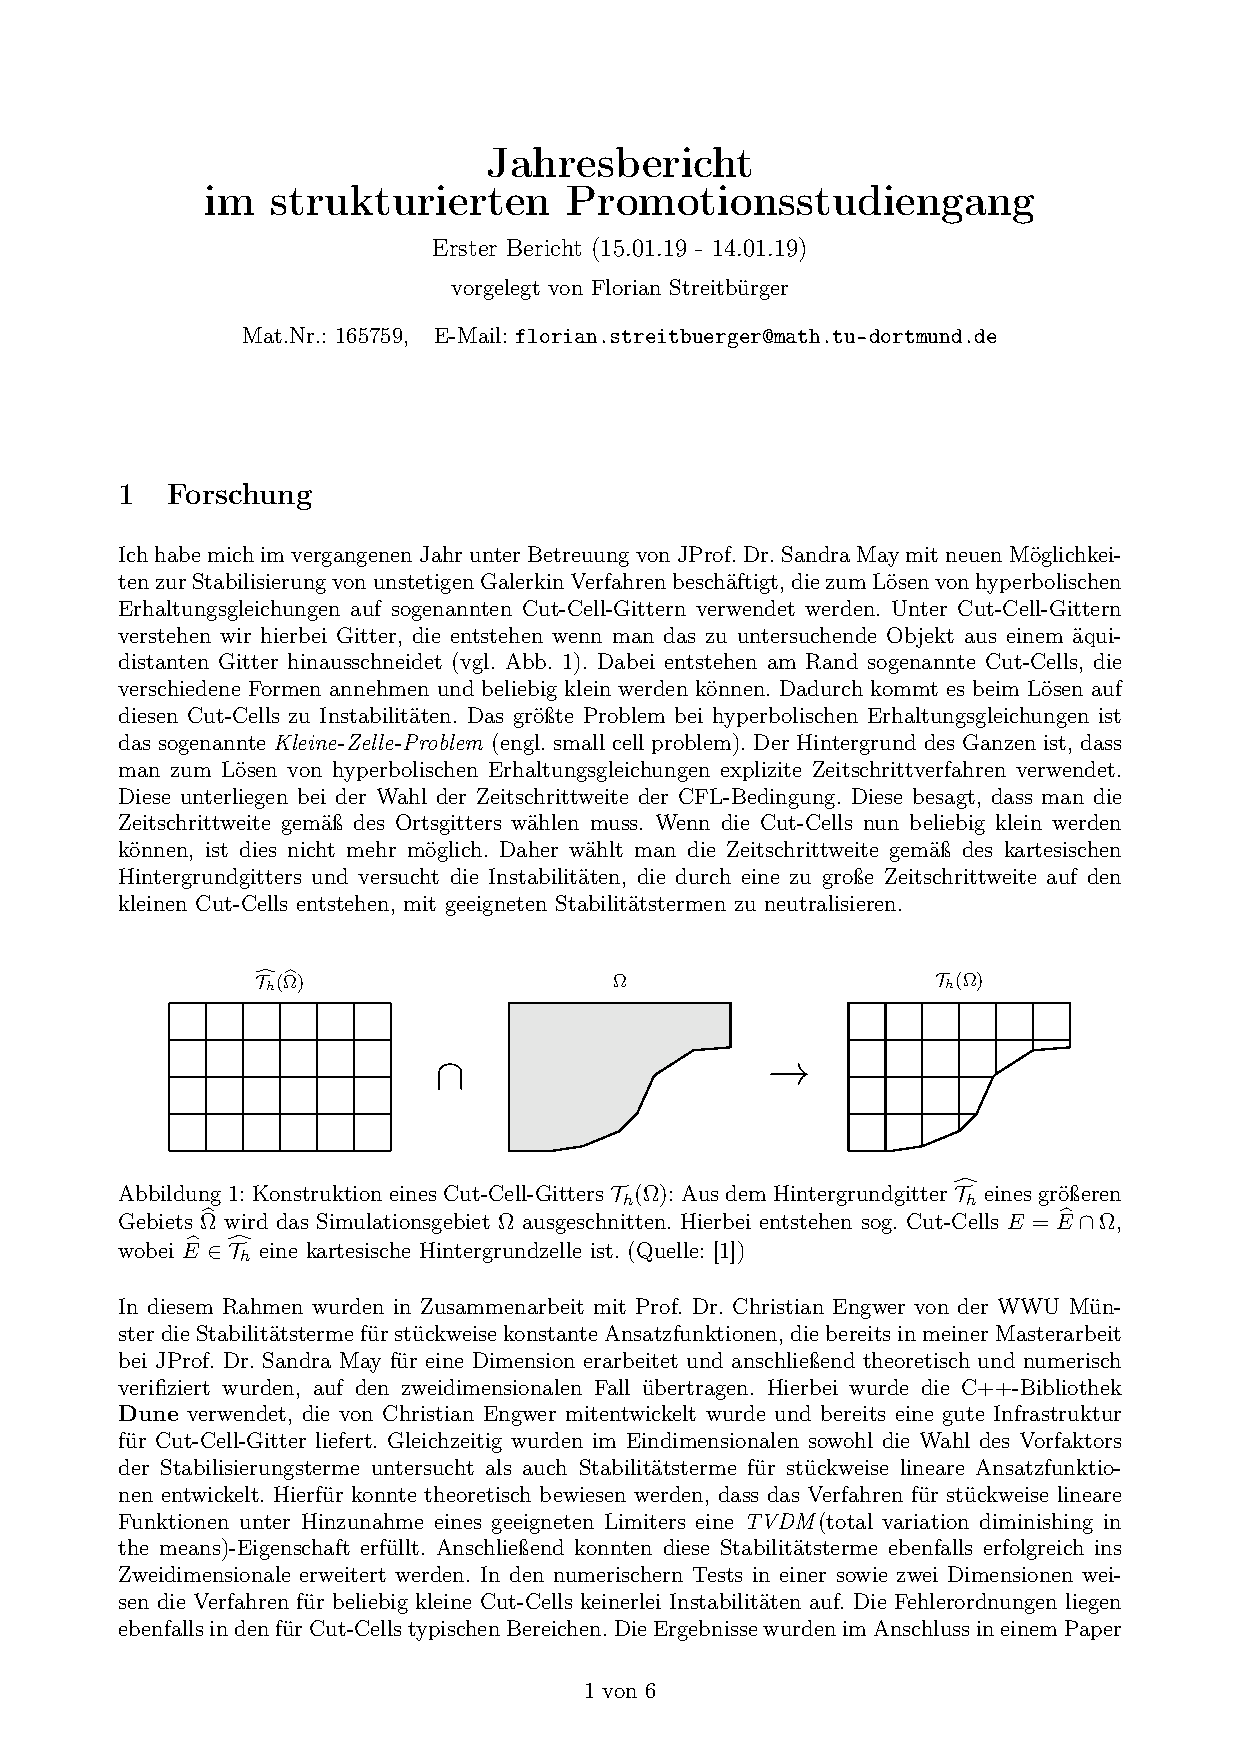
\includepdf[pages=1-4]{Jahresbericht-1.pdf}
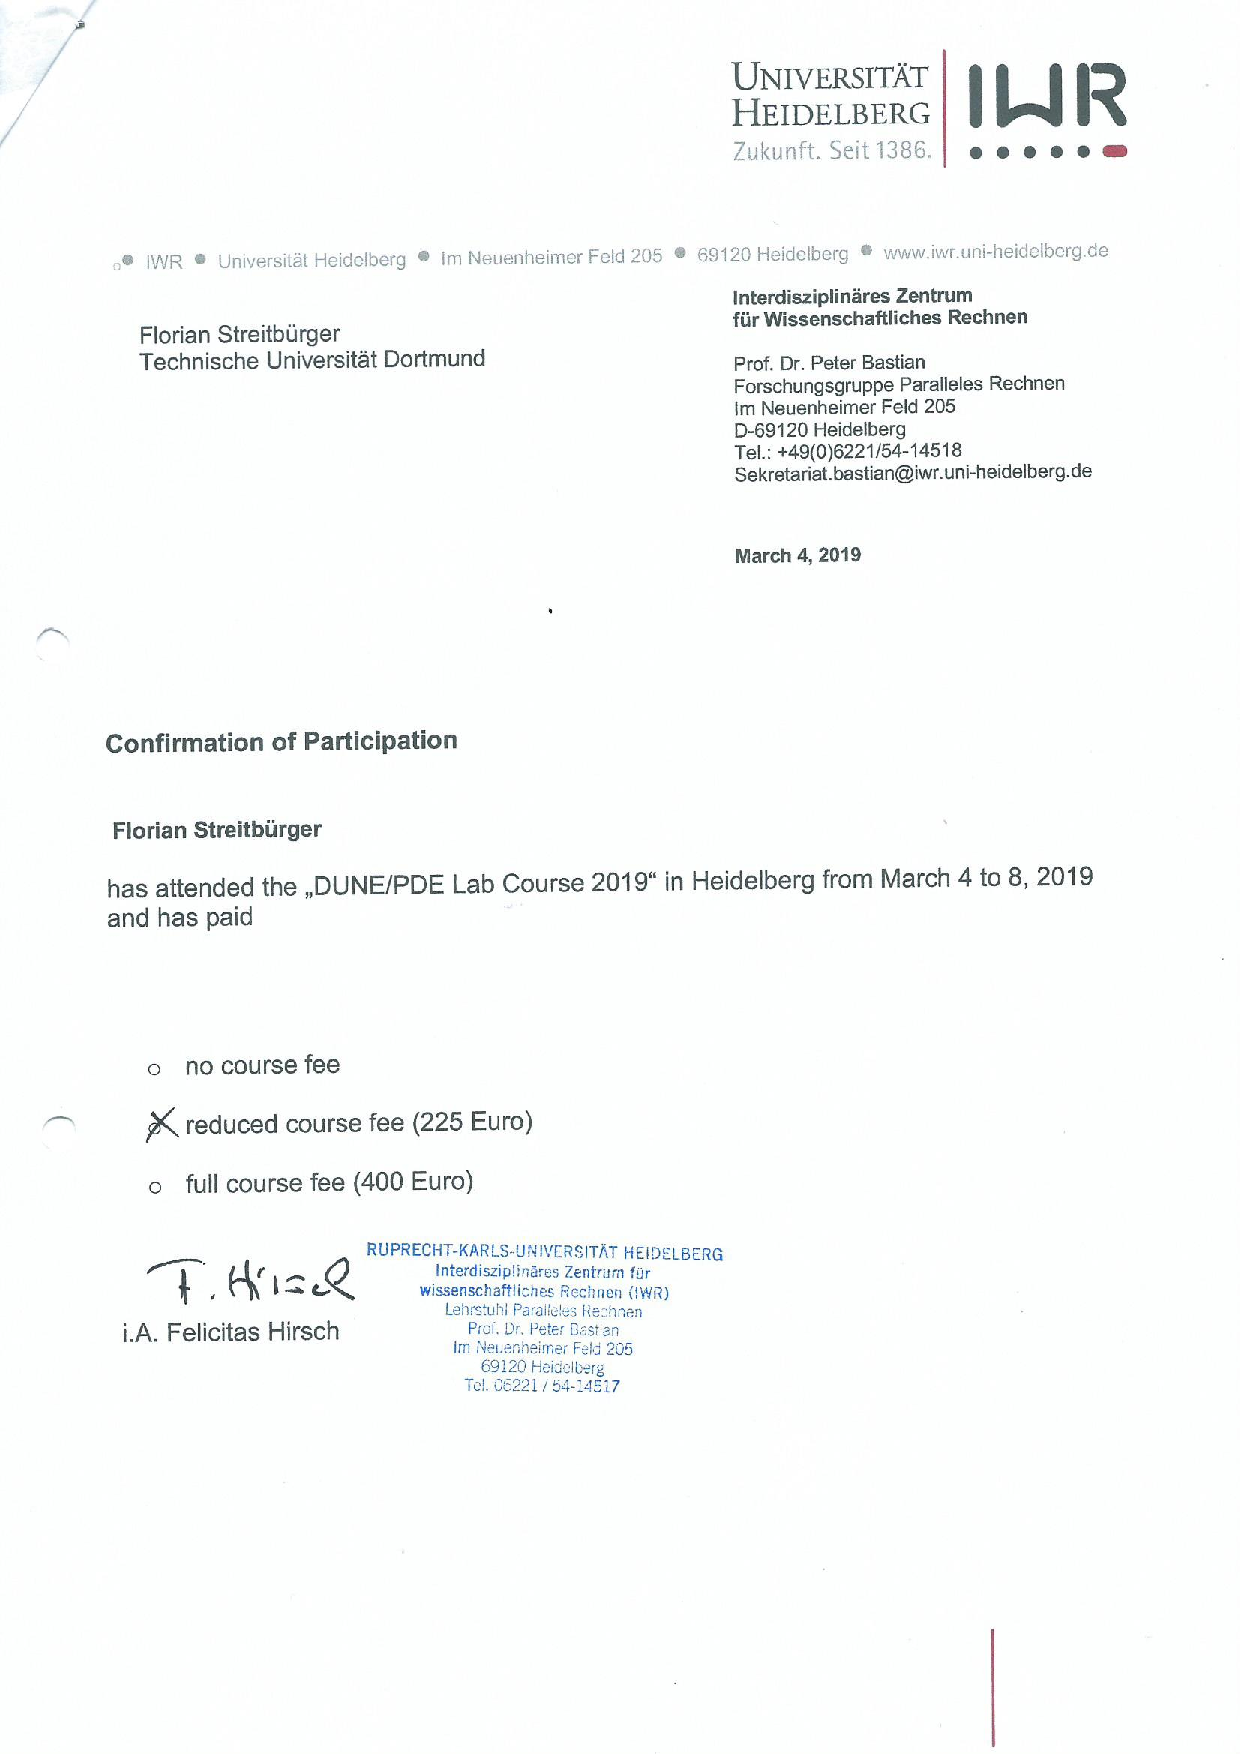
\includepdf[pages=1]{DUNE_Kurs.pdf}
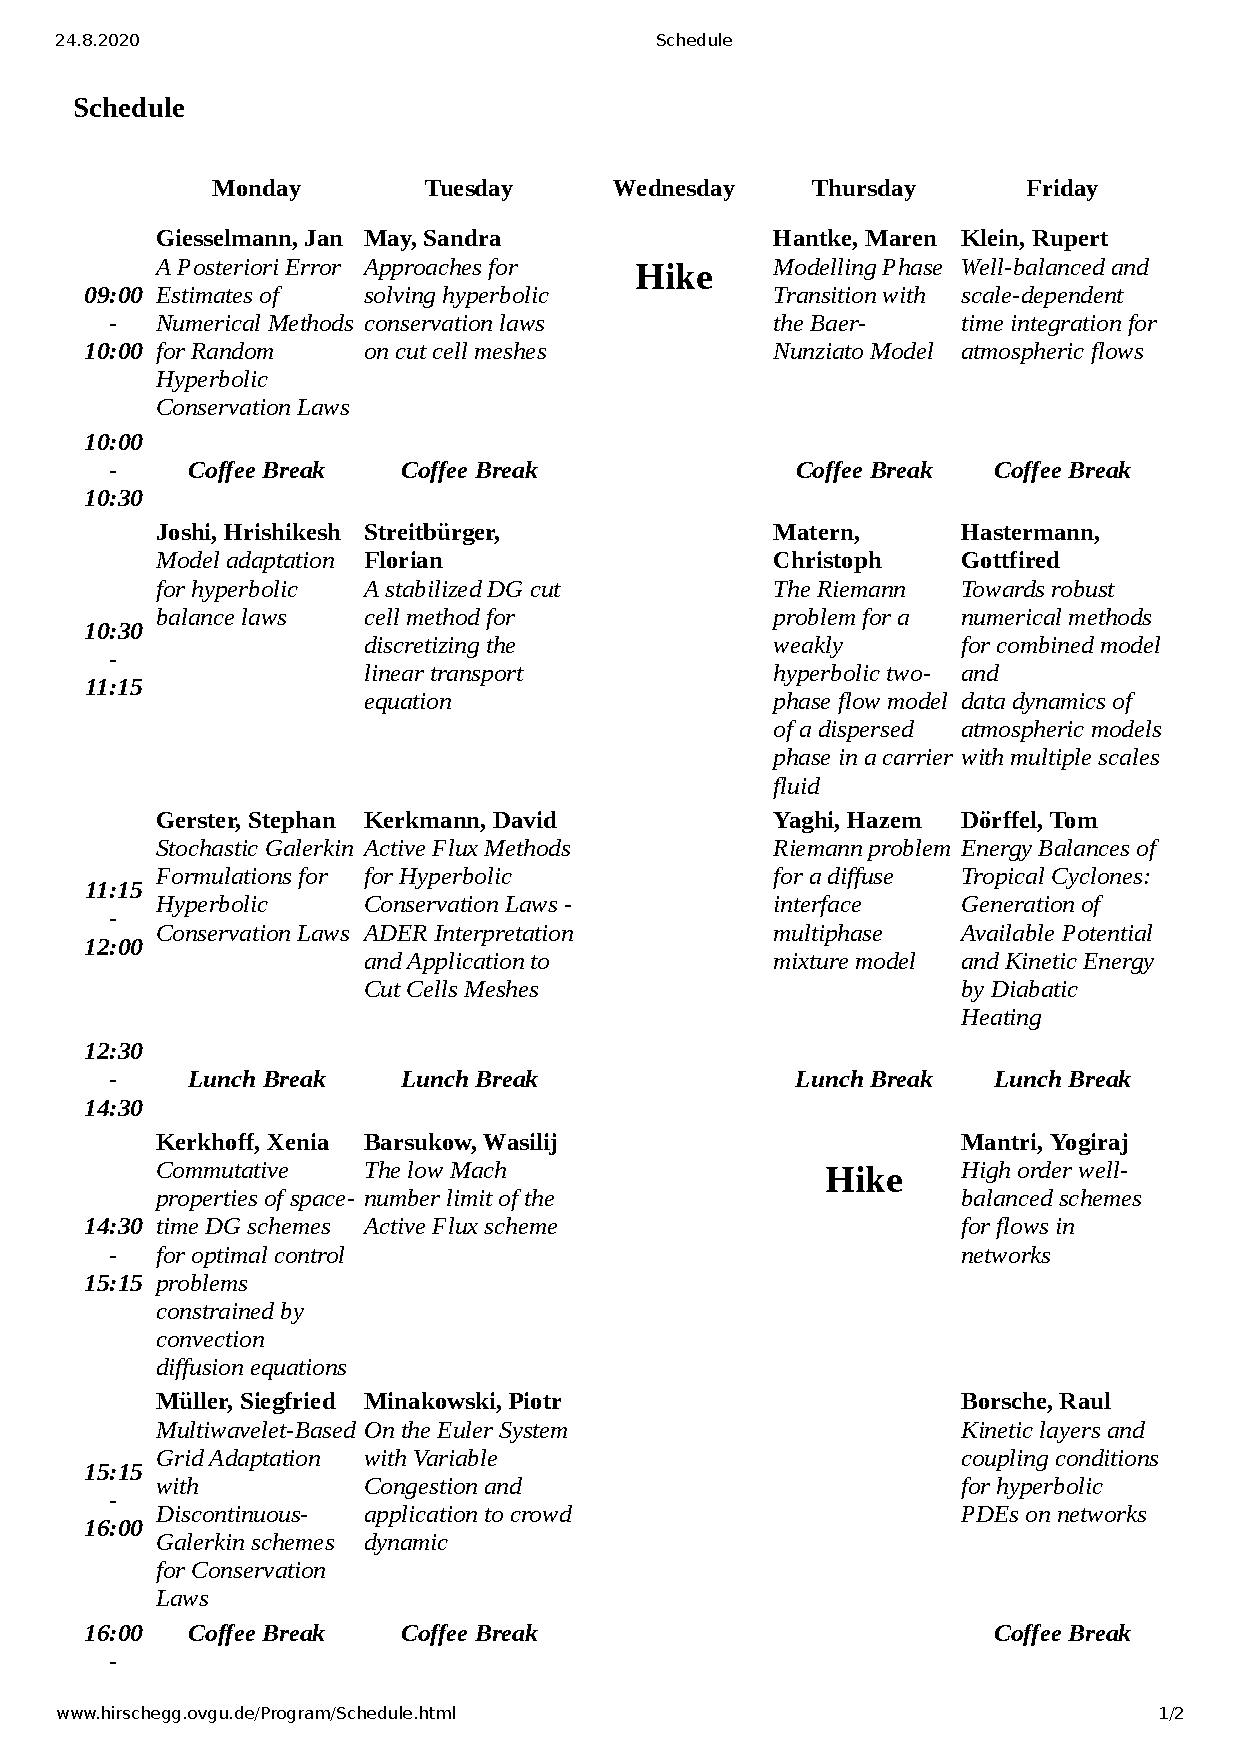
\includepdf[pages=1-2]{Program_Hirschegg}
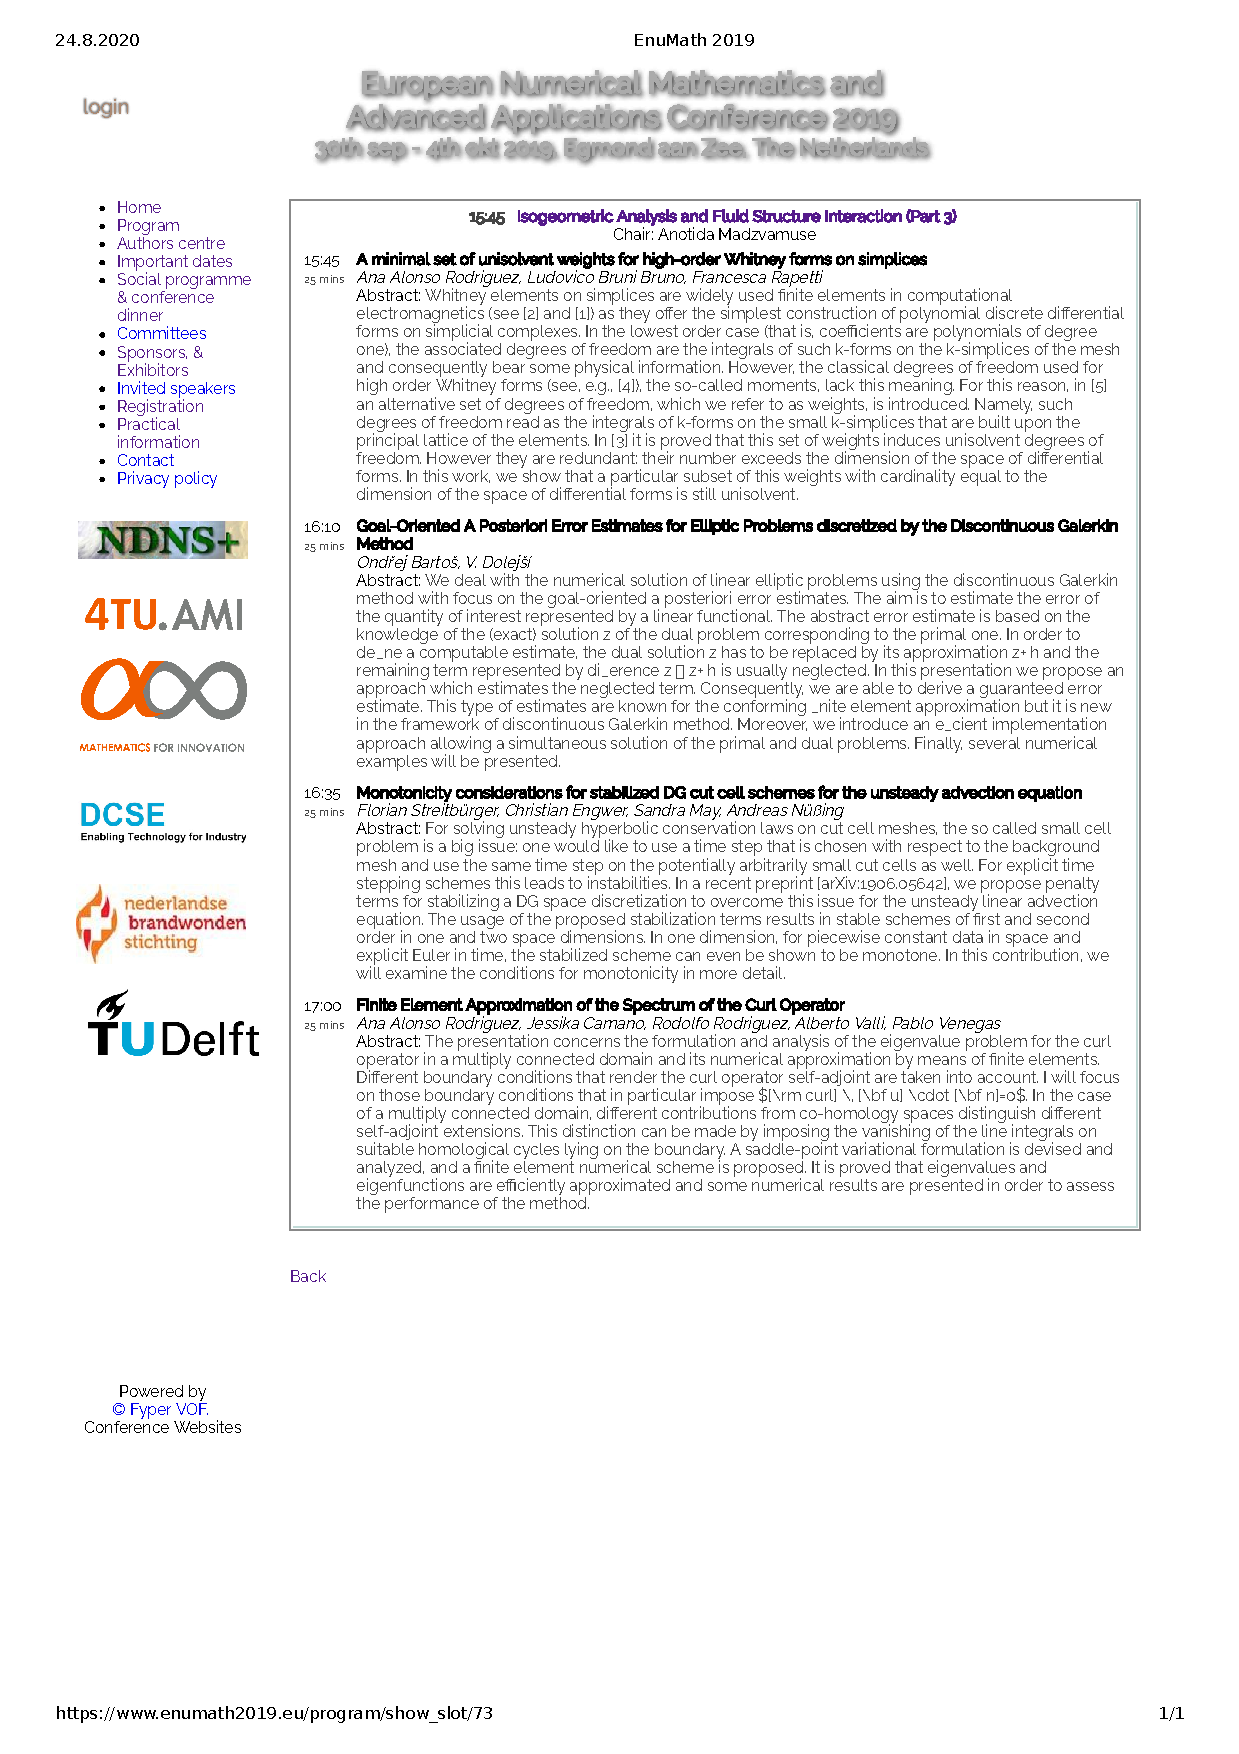
\includepdf[pages=1]{EnuMath2019_Programm}

\includepdf[pages=1]{Oberseminar_LSIII}
\includepdf[pages={6,49}]{OberwolfachReport_2019_No24}
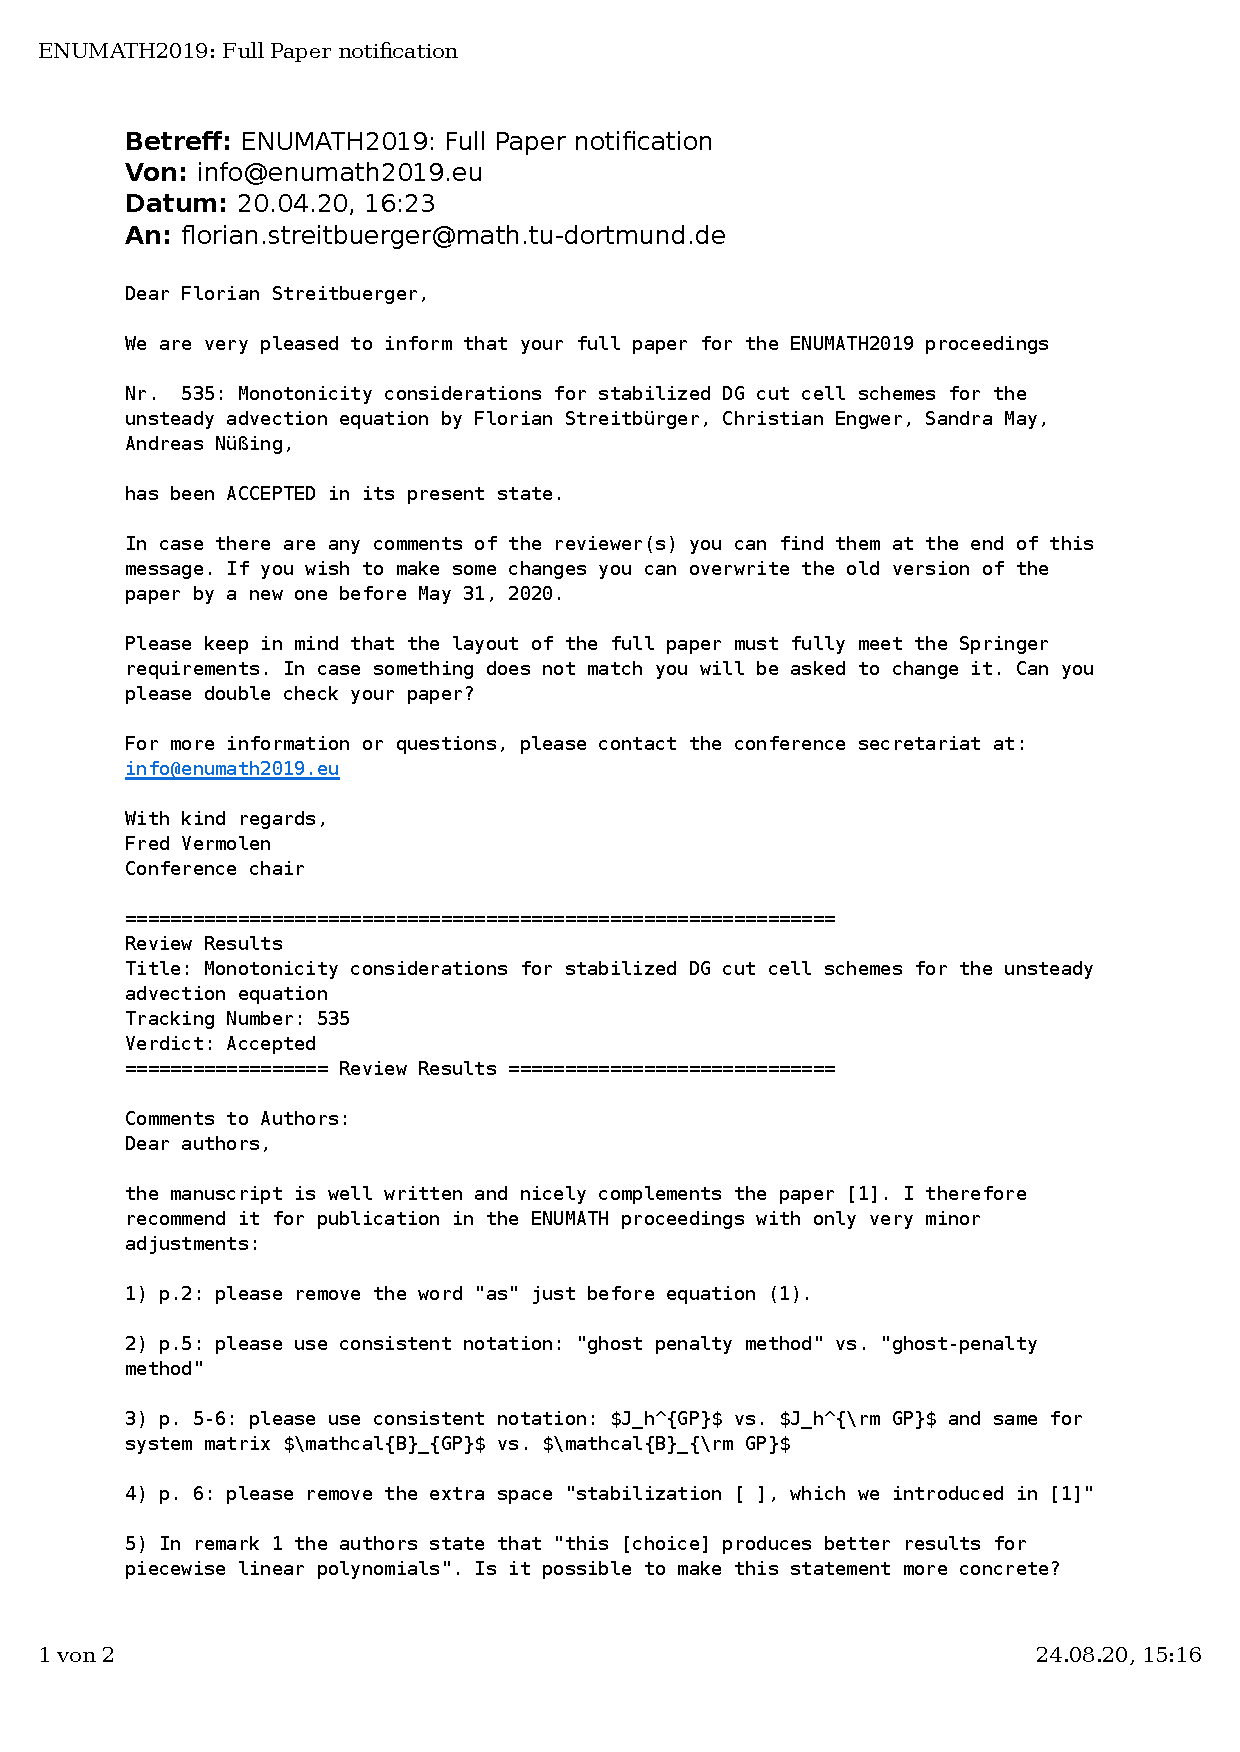
\includepdf[pages=1-2]{EnuMath2019_submission}
\end{document}

